%!TEX root = perrinet20cnrs.tex
%!TeX TS-program = Lualatex
%!TeX encoding = UTF-8 Unicode
%!TeX spellcheck = fr-FR
%!BIB TS-program = biber
% -*- coding: UTF-8; -*-
% vim: set fenc=utf-8
\documentclass[11pt,french,a4paper,oneside]{article}%,twoside,draft
%============ common ===================
\usepackage[utf8]{inputenc}%
\usepackage[french]{babel}%
\usepackage{csquotes}%
\usepackage{etaremune}%
\usepackage[final]{pdfpages}%
%% --- unit formatting ---
\usepackage{microtype}	% Better typography \tolerance 1414
\hbadness 1414
\emergencystretch 1.5em
\hfuzz 0.3pt
\widowpenalty=10000
\vfuzz \hfuzz
\raggedbottom
%%%%%%%%%%%%%%%%%%%%%%%%%%%%%%%%%%%%%%%%%%%%%%%%%%%%%%%%%%%%%%%%%%%%%
\usepackage{amsmath,amsfonts,amsthm}			% Math packages
\usepackage{bm}%This package defines commands to access bold math symbols
\usepackage{graphicx}					% Enable pdflatex
%============ front-matter ===================
\newcommand{\BookTitle}{Centre National de la Recherche Scientifique
\\
{\sc Programme de recherche}

}
\newcommand{\Title}{%
La vision comme processus prédictif: Une approche bio-mimétique.
}%
\newcommand{\Resume}{%
Mon programme de recherche s'articule autour de l'hypothèse que la dynamique de la vision est un processus prédictif. Cette hypothèse permet alors de construire une architecture innovante de calcul que nous appliquerons à un modèle du cortex visuel primaire. La démarche qui est suivie est de confronter directement ces modèles en testant leurs prédictions avec des expériences neurophysiologiques, notamment sur le caractère impulsionnel et parcimonieux du code neural. L'objectif est à la fois une meilleure compréhension des mécanismes neuraux dans les aires visuelles primaires mais aussi l'application de ces principes computationnels pour créer de nouveaux paradigmes computationnels en vision par ordinateur. En se focalisant sur cette approche bio-mimétique, l'ambition à long terme est de dépasser les limites des réseaux de neurones convolutionnels profonds actuels et créer une nouvelle génération de réseaux de neurones artificiels.
}%
\newcommand{\Keywords}{%
Vision; Biomimetics; Predictive processes; Computational Neuroscience; Artificial Intelligence
}%
\newcommand{\SubTitle}{%
Pour évaluation par les sections du Comité national}%
\newcommand{\Author}{Laurent U.~Perrinet}%
\newcommand{\Team}{\'Equipe NEural OPerations in TOpographies (NeOpTo)}%
\newcommand{\Institute}{Institut de Neurosciences de la Timone}%
\newcommand{\InstituteUMR}{UMR 7289, CNRS / Aix-Marseille Université}%
\newcommand{\Address}{27, Bd. Jean Moulin, 13385 Marseille Cedex 5, France}
\newcommand{\Website}{https://laurentperrinet.github.io/}
\newcommand{\Email}{Laurent.Perrinet@univ-amu.fr}
%%%%%%%%%%%%%%%%%%
%BIBLIOGRAPHY
%%%%%%%%%%%%%%%%%%
\usepackage[natbib=true,
			bibencoding=utf8,
%			encoding=utf8,
			maxcitenames=7,
			maxnames=7,
			%minnames=3,
			maxbibnames=7,
            sortcites=true,
            block=space,
            backend=biber,
%            doi=false,isbn=false,url=false,
            citestyle=alphabetic,%authoryear-comp,
            backref=true,
%            bibstyle=alphabetic
            ]{biblatex}%
\addbibresource{Perrinet20PredictiveProcessing.bib}
\addbibresource{babel.bib}
\addbibresource{~/metagit/blog/perrinet_curriculum-vitae_tex/LaurentPerrinet_Publications.bib}
\addbibresource{~/metagit/blog/perrinet_curriculum-vitae_tex/LaurentPerrinet_Presentations.bib}
%\usepackage[normalem]{ulem} %for \uline{}
%\DeclareNameFormat{given-family}{
%  \ifgiveninits
%  {\ifthenelse{\equal{\namepartfamily}{Toto}}
%    {\uline{\namepartfamily\addspace\namepartgiveni\namepartsuffix}}
%    {\namepartfamily\addspace\namepartgiveni\namepartsuffix}
%    \ifthenelse{\value{listcount} < \value{liststop}}
%    {\addcomma}
%    {\ifthenelse{\ifmorenames}{~et \,al \adddot}}
%    {}
%  }
%}
% https://tex.stackexchange.com/questions/359311/how-to-underline-name-of-specific-authors-in-biblatex
\usepackage{xpatch}
\usepackage[normalem]{ulem}

\newbox\savenamebox

%\newbibmacro*{name:bbold}[2]{%
%  \def\do##1{\iffieldequalstr{hash}{##1}{\bfseries\setbox\savenamebox\hbox\bgroup \listbreak}{}}%
%  \dolistloop{\boldnames}%
%}
\newbibmacro*{name:bbold}[2]{%
  \def\do##1{\iffieldequalstr{hash}{##1}{\setbox\savenamebox\hbox\bgroup \listbreak}{}}%
  \dolistloop{\boldnames}%
}

\newbibmacro*{name:ebold}[2]{%
  \def\do##1{\iffieldequalstr{hash}{##1}{\egroup\uline{\usebox\savenamebox}\listbreak}{}}%
  \dolistloop{\boldnames}%
}

\xpatchbibmacro{name:given-family}{\usebibmacro{name:delim}{#2#3#1}}{\usebibmacro{name:delim}{#2#3#1}\begingroup\usebibmacro{name:bbold}{#1}{#2}}{}{}

%\xpretobibmacro{name:given-family}{\begingroup\usebibmacro{name:bbold}{#1}{#2}}{}{}
\xapptobibmacro{name:delim}{\begingroup\normalfont}{}{}

\xapptobibmacro{name:given-family}{\usebibmacro{name:ebold}{#1}{#2}\endgroup}{}{}
\xapptobibmacro{name:delim}{\endgroup}{}{}

\newcommand*{\boldnames}{}
\forcsvlist{\listadd\boldnames}{
  {8fa031352aa34db95f5c1022358042a3}, % InBold
  {01b588ba4e4ad753feae6c81709fc04b}} % Highlight

%%%%%%%%%%%%%%%%%%%%%%%%%%%%%%
%% OPTIONAL MACRO FILES
%\usepackage{fltpage}
%\usepackage{tikz}
%%%%%%%%%%%%%%%%%%
%\usepackage{multicol}
%\usepackage{nag}
%============ graphics ===================
\usepackage{graphicx}
%============ hyperref ===================
\usepackage[unicode,linkcolor=blue,citecolor=blue,filecolor=black,urlcolor=blue,%pdfborder={0 0 0}
]{hyperref}%
\hypersetup{%
unicode = true, %
pdftitle={\Title},%
pdfauthor={\Author < \Email > - \Institute, \InstituteUMR , \Address - \Website},%
pdfsubject={\Title}%
}%
%\hypersetup{linkcolor=blue,citecolor=blue,filecolor=black,urlcolor=blue}
%\hyphenpenalty=5000
%\tolerance=1000
%% DOCUMENT LAYOUT
%\usepackage{geometry}
%\geometry{a4paper, textwidth=5.5in, textheight=8.5in, marginparsep=7pt, marginparwidth=.6in}
%\setlength\parindent{0in}
%% ---- MARGIN YEARS
\newcommand{\years}[1]{\marginpar{\textit{\scriptsize #1}}}
\providecommand{\natexlab}[1]{#1}
%\providecommand{\url}[1]{\texttt{#1}}
%\expandafter\ifx\csname urlstyle\endcsname\relax
 \providecommand{\doi}[1]{doi: #1}%\else
%  \providecommand{\doi}{doi: \begingroup \urlstyle{rm}\Url}\fi
%\makepagestyle{chapter}
%\makeoddfoot{chapter}{\addRevisionData}{\thepage}{}
%\makeevenfoot{chapter}{\addRevisionData}{\thepage}{}
\graphicspath{{./../2020-07-06_Perrinet20PredictiveProcessing/figures/}}%
%\graphicspath{{figures/}}%,{./khoei13jpp/figures/},{./bednar/},{./kaplan13/},{./friston/},{../../sci/dyva/lup/Learning/mp_sparsenet/mp_sparsenet/results/20080502T174325}}%
%%%%%%%%%%%% Her begynner selve dokumentet %%%%%%%%%%%%%%%

% for units
\usepackage{siunitx}%
\newcommand{\ms}{\si{\milli\second}}%

\usepackage{geometry}
\geometry{hscale=0.66,vscale=0.8,centering}

\begin{document}

\begin{titlepage}

\begin{center}
%\vskip 2cm
\emph{\Large \BookTitle }%
\vskip 2cm
{\Huge \Title}
\vskip 1cm
{\Large Laurent \textsc{Perrinet}}
\vskip 1cm
\emph{\Large \SubTitle }\\%
%\begin{tabular}[t]{ccc}
%\includegraphics[height=2.5cm]{logo_cnrs-UAM.png} &%\includegraphics[]{}
%\includegraphics[height=2.5cm]{logo_int.png} %& %
%%	\includegraphics[height=2.5cm]{U2_logo.pdf}
%\end{tabular}
\vskip 1cm
\includegraphics[width=1.\textwidth]{/Users/laurentperrinet/quantic/libraries/slides.py/figures/troislogos.png}
\vskip 1cm
\begin{tabular}[t]{|c|}
\hline
\Team \\\hline
\Institute \\ \InstituteUMR \\\hline
\Address \\\hline
\url{\Website}\\\hline
\url{\Email}\\\hline
\end{tabular}
\vskip .5cm
\vfill
{\large 7 janvier 2020}
\end{center}
\end{titlepage}

%%%%%%%%%%%% Endyet daag koepf dokumentet %%%%%%%%%%%%%%%
\begin{abstract}
% TODO :Dans un souci d’homogénéisation, la Section appréciera que chacun des 2 dossiers « Travaux antérieurs » et « Projet de recherche » compte entre 15 et 20 pages au maximum (taille de caractères 12, interligne 1,5).
\Resume
%
%26/01
%DR2
%
%26
%	Cerveau, cognition, comportement

%51/01
%DR2
%	Modélisation et analyse des données et des systèmes biologiques : approches informatiques, mathématiques et physiques
%

%Ce rapport est l'occasion de faire le point sur un travail scientifique depuis ma soutenance d'habilitation à diriger des recherches en 2014 en focalisant sur les cinq derniers semestres (de mars 2017 à septembre 2019).

%La première partie résume ce parcours : l
%Le Chapitre~\ref{chap:projet} présente mon programme de recherche, tandis que le chapitre~\ref{chap:cv} détaille mon CV et le chapitre~\ref{chap:publis} comprend la liste exhaustive de mes publications.

%La dernière partie du manuscrit (Chapitre 6) présente enfin une description des perspectives de cette démarche scientifique.

\end{abstract}
\newpage
\tableofcontents
\newpage
%%%%%%%%%%%%%%%%%%%%%%%%%%%%%%%%%%%%%%%%%%%%%%%%%%%%%%%%%%%
%!TEX root = perrinet20cnrs.tex
%!TeX TS-program = Lualatex
%!TeX encoding = UTF-8 Unicode
%!TeX spellcheck = fr-FR
%!BIB TS-program = bibtex
% -*- coding: UTF-8; -*-
% vim: set fenc=utf-8
%\chapter{Programme de recherche: La dynamique de la vision est un processus prédictif}
% Pour chaque concours auquel vous postulez, saisissez l'intitulé et le résumé de votre programme de recherche ; vous pouvez aussi joindre le document de votre projet de programme de recherche.
% Intitulé du programme de recherche proposé / Résumé / 5 mots clés
%\label{chap:projet}%

Au sein du système nerveux central, les aires visuelles sont
essentielles pour transformer le signal lumineux brut en une
représentation qui transmet efficacement des informations sur
l'environnement. Ce processus est modelé par la nécessité d'être robuste
et rapide. En effet, il existe d'un coté une grande variété de
changements possibles dans les caractéristiques géométriques de la
scène visuelle et de l'autre, il existe une urgence continue d'être capable de répondre à chaque instant et le plus rapidement
possible au flux sensoriel entrant, par exemple pour entraîner un
mouvement des yeux vers l'emplacement d'un danger potentiel. Des
décennies d'études en neurophysiologie et en psychophysique aux
différents niveaux de vision ont montré que de nombreuses facettes de ce système tirent profit des
connaissances a priori sur la structure de l'information visuelle,
telles que la régularité dans la forme et le mouvement des objets
visuels. Ainsi, le cadre du \emph{traitement prédictif} offre une théorie
unifiée pour expliquer une large variété de mécanismes visuels. Toutefois, \textbf{il
nous manque encore une approche normative globale unifiant les
processus visuels.}

\textbf{Le projet de recherche que j'ai développé
explore la dynamique du traitement prédictif dans le système visuel,
de la rétine à l'action.}
Afin de le définir, nous passerons rapidement en revue ici quelques approches récentes et
prometteuses auxquelles j'ai eu la chance de contribuer. Tout d'abord, nous décrirons l'inférence active, une forme
de traitement prédictif doté de la capacité d'échantillonner activement
l'espace visuel. Ensuite, nous étendrons ce paradigme au cas où
l'information est distribuée sur une topographie, comme c'est le cas
pour les aires visuelles organisées rétinotopiquement. En particulier,
nous comparerons ces modèles à la lumière de données neurophysiologiques
récentes montrant le rôle des vagues d'activation dans la formation du
traitement visuel. Enfin, \textbf{je vais proposer un programme de recherche original
pour comprendre comment ces modèles fonctionnels peuvent être mis en
œuvre au niveau neural sous la forme de cartes topographiques adaptatives de micro-circuits
prototypiques}. Ceux-ci permettent de séparer les différents flux
d'information, depuis l'erreur de prédiction sensorielle à l'erreur d'anticipation de la rétroaction.
Néanmoins, la conception d'un tel
circuit de traitement prédictif générique est un champ de recherche ouvert et nous énumérerons quelques implémentations possibles à l'aide
de réseaux de neurones biomimétiques.

\section{Motivation : Dynamique des calculs neuronaux
sous-jacents au traitement
visuel}
La vision, c'est-à-dire la capacité de donner un sens à l'environnement
lumineux, est traditionnellement considérée comme une séquence d'étapes
de traitement allant de l'entrée rétinienne à une représentation de
niveau supérieur, permettant éventuellement une action. On pense souvent que cette séquence d'étapes de
traitement, ou ``pipeline'', est mise en œuvre par un
processus ``feed-forward'' (en avant) dans les voies visuelles, à travers le thalamus
et ensuite dans les aires visuelles du cortex cérébral. Un tel modèle de
vision est suffisant pour expliquer la simple détection du caractère
imprimé que vous êtes en train de regarder, et donc pour la lecture
d'une phrase complète. En effet, une telle capacité implique des
processus de bas niveau rapides et inconscients. Il est important de
noter que cette aptitude chez l'homme est également largement robuste
aux changements de luminance (comme une ombre sur cette page) ou
aux déformations géométriques, comme lors de la lecture de ce
texte dans une perspective inclinée. Plus généralement, la vision biologique
complétera correctement l'image d'un mot avec des lettres manquantes ou
avec des détections ambiguës ou incorrectes dues à une occlusion ou un
chevauchement. Une telle robustesse est caractéristique des systèmes
biologiques, d'où son utilisation comme test de Turing pour les
algorithmes de sécurité tels que les
\href{https://fr.m.wikipedia.org/wiki/CAPTCHA}{CAPTCHAs}.
De manière générale, les modèles de vision tels qu'ils sont mis en œuvre dans les ordinateurs
peuvent apprendre de telles tâches sur des
ensembles de données très précis.
Par exemple, des réseaux de neurones artificiels de type ``apprentissage profond'' ont récemment prouvé qu'ils pouvaient dépasser la performance humaine sur une tache de catégorisation d'images statiques~\citep{NIPS2012_4824}. %, ou pour jouer au jeu de Go~\citep{Silver16}.
Toutefois, ces mêmes processus sont facilement surpassés par un
enfant de 6 ans lorsqu'il s'agit d'un contexte écologique, flexible et
générique. En allant encore plus loin, la vision humaine se caractérise
aussi par des processus de plus haut niveau et permet des prédictions
prospectives telles que celles révélées par l'imagerie mentale - et
constitue la pierre angulaire de la créativité, ou de
son \emph{imagination}. La vision est donc un processus
extrêmement complexe, et les étapes de traitement ne sont sûrement pas indépendantes. %: mais elle n'est pas encore complètement comprise.
En fait, le plus surprenant au sujet de la vision est la
facilité avec laquelle les personnes voyantes peuvent apprendre à exercer ces
capacités. Pour reformuler~\citet{Wigner90}, ``l'efficacité déraisonnable de
la vision dans le monde naturel'' nous invite à nous concentrer sur cette
capacité cognitive pour une meilleure compréhension du cerveau en
général.

Anatomiquement, la vision est le résultat de l'interaction de réseaux
neuronaux qui sont organisés en une hiérarchie d'aires visuelles.
Chaque aire visuelle est un processus dynamique, depuis sa
première étape, la rétine, jusqu'aux aires visuelles efférentes qui
contribuent à former une représentation parallèle et distribuée du monde
visuel. De plus, cette organisation est largement auto-organisée et très
efficace sur le plan métabolique. Pour comprendre le fonctionnement d'un réseau aussi
complexe d'aires visuelles, il a été proposé que ce système soit
organisé de manière à \emph{prédire} efficacement les données
sensorielles~\citep{Attneave54}. Cette approche écologique~\citep{Atick92}
permet d'expliquer de nombreux aspects de la vision comme traitement
prédictif. Une telle approche prend différentes formes telles que la
réduction de la redondance~\citep{Barlow61}, la maximisation du transfert
d'information~\citep{Linsker90} ou la minimisation de l'énergie
métabolique. La formalisation de ces stratégies d'optimisation en
langage probabiliste peut être englobée dans le cadre du ``cerveau
Bayesien''~\citep{Knill04}. Plus généralement, il est possible de
relier ces différentes théories dans un cadre unique, le principe de
l'énergie libre (Free-Energy Principle, FEP)~\citep{Friston10}. Ce principe constitue un
changement de paradigme crucial pour l'étude des processus prédictifs
tant au niveau philosophique que scientifique. La clé de ce principe est
la notion que, connaissant les processus qui ont généré l'image visuelle
et le modèle de génération interne qui permet sa représentation, les
processus prédictifs profiteront de la connaissance \emph{a priori} pour
former une représentation optimale de la scène visuelle~\citep{Rao99}. Cette connaissance constitue une représentation explicite
(probabiliste) de la structure du monde. Par exemple, une image composée
de bords sera comprise à un niveau supérieur dans la hiérarchie visuelle en utilisant la
connaissance a priori du lien entre les bords individuels pour former
une représentation des \emph{contours} des objets visuels. Dans le
domaine temporel, la connaissance des transformations géométriques
telles que le mouvement des objets visuels aidera à prédire leur
position future et à suivre les différents segments du mouvement, mais aussi
à représenter les contours invariablement à ce mouvement.

Cependant, il y a des limites et des contraintes à l'efficacité de la
vision. Premièrement, l'information lumineuse peut être bruitée et
ambiguë, par exemple dans des conditions de faible luminosité. Cela
contraint le système à être robuste face aux incertitudes. Cela met en
évidence un avantage clé du traitement prédictif, car il implique
l'apprentissage d'un modèle génératif des données sensorielles. D'une
part, en représentant explicitement la précision des variables
(l'inverse de la variance inférée de sa valeur), on peut intégrer de
manière optimale des informations distribuées, même dans le cas où cette
incertitude n'est pas uniforme et évolue dynamiquement dans le système.
D'autre part, un modèle génératif permet de représenter explicitement
les transformations des données (comme une transformation géométrique de
l'image comme une translation ou une rotation) et donc de faire des
prédictions sur les états futurs. Deuxièmement, les réseaux neuronaux
ont des capacités limitées de transfert de l'information et ont toujours
besoin d'un certain délai pour transmettre et traiter l'information.
Chez l'humain, par exemple, le délai de transmission de l'information
rétinienne au cortex est d'environ 50~\ms, tandis que la latence minimale
pour effectuer une action oculomotrice est d'environ 50~\ms~\citep{Kirchner06}
 (voir~\citep{Lamme00} pour des valeurs
équivalentes chez le singe). Bien que cela limite naturellement la
capacité du système visuel, nous profiterons ici de ces délais pour
disséquer les différents processus visuels. {\bf En particulier, nous nous
concentrerons dans ce programme de recherche sur ma contribution dans l'étude
du rôle de ces contraintes
temporelles sur la dynamique des processus prédictifs}.

Pour illustrer le défi de représenter un signal dynamique, prenons
l'exemple de l'enregistrement d'un ensemble de cellules neurales dans
certaines aires visuelles. Supposons que ces enregistrements soient
évoqués par un signal visuel analogique (comme un signal lumineux
projeté sur une population de cellules sensorielles rétiniennes) et que
l'on puisse extraire les temps exacts des événements de décharge
pour une population de cellules. Nous pouvons ensuite choisir d'afficher
ces données sur une figure sous forme de ``tracé temporel'', c'est-à-dire de montrer le moment
des spikes pour chacune des cellules identifiées. Le temps est donc
relatif à celui de l'expérimentateur et est donné grâce à une horloge
externe : Il est montré \emph{a posteriori}, c'est-à-dire après
l'enregistrement. En général, cette définition d'un temps absolu a
d'abord été formalisée par Newton et définit la plupart des lois de la
physique, utilisant le temps comme un paramètre externe. Mais il n'y a
encore aucune preuve que les neurones auraient accès à une horloge
centrale qui donne accès à l'heure physique absolue. Au
contraire, les réponses neurales sont uniquement contrôlées par la
distribution \emph{actuelle} des gradients électrochimiques sur leur
membrane, potentiellement modulés par les cellules voisines. Une telle
notion du temps est propre à chaque neurone et à son environnement. En
conséquence, la dynamique du réseau est largement asynchrone,
c'est-à-dire que le ``chronométrage'' est décentralisé. De plus, cette
notion locale de temps (de traitement) est \emph{a priori} disjointe du
temps externe qui est utilisé pour représenter le signal visuel. Une
telle observation est essentielle pour comprendre les principes qui
guident l'organisation des processus visuels : Une théorie neurale des
processus prédictifs ne peut être définie que dans ce temps local, en utilisant uniquement les informations disponibles
localement et à l'instant présent. En particulier, nous proposerons que les
processus neuronaux en vision visent à ``prédire le présent''~\citep{Changizi08} en utilisant un modèle générateur interne de la scène visuelle
et en utilisant des données sensorielles pour valider cette
représentation interne.

Ce programme de recherche passe en revue ces approches de traitement prédictif
dynamique pour la vision à différentes échelles d'analyse, de l'ensemble
du système aux représentations intermédiaires et enfin aux neurones (en
suivant dans un ordre décroissant les niveaux d'analyse de~\citet{Marr83}).
Tout d'abord, nous appliquerons la FEP à la vision en tant qu'approche
normative. De plus, les représentations visuelles doivent prendre en
charge les transformations géométriques (comme le mouvement d'un objet
visuel) mais aussi les modifications sensorielles, comme les mouvements
des yeux. En étendant le principe précédent à la capacité
d'échantillonner activement les données sensorielles, nous définirons
l'inférence active (IA) et illustrerons son rôle potentiel dans la
compréhension de la vision, ainsi que des comportements comme les
mouvements oculaires. Ensuite, nous l'étendrons pour
comprendre comment de tels processus peuvent être mis en œuvre sur des
cartes rétinotopiques. En particulier, nous montrerons
comment un tel modèle peut expliquer une illusion visuelle, l'effet du flash retardé. %Flash-lag.
Ces données seront ensuite comparées aux données
neurophysiologiques. Enfin, nous examinerons les implémentations
possibles de tels modèles dans les réseaux de neurones impulsionnels. En particulier, nous passerons en revue quelques modèles de
micro-circuits élémentaires et détaillerons quelques règles potentielles
pour apprendre la structure de leurs connexions d'une manière non
supervisée. Nous pourrons ainsi conclure en dessinant les perspectives de résultats de ce programme de recherche.

\section{L'inférence active et ``l'optimalité de la vision''}
\label{sec:ai}
Les principes d'optimisation semblent le seul choix pour comprendre
``L'efficacité déraisonnable de la vision dans le monde naturel''.
Cependant, essayer de comprendre la vision comme un processus émergent
d'un principe d'optimisation semble être un principe téléologique dans
lequel la causalité serait inversée~\citep{Turkheimer19}. Pourtant,
``l'utilisation du principe téléologique n'est qu'un moyen, et non la
totalité ou l'unique, par lequel nous pouvons chercher à apprendre
comment les choses sont apparues et ont pris leur place dans la
complexité harmonieuse du monde.''~\citep[chap. 1, ma traduction]{DArcy-Thompson17}. En
d'autres termes, il n'est pas important d'un point de vue scientifique
de savoir si le cerveau utilise explicitement un tel principe (par
exemple que certaines de ses parties puissent utiliser la règle de
Bayes), mais plutôt qu'un tel ensemble de règles offre une explication
plus simple des enregistrements neuraux en mettant en lumière les
processus se produisant dans ce système complexe~\citep{Varoquaux19}.
Nous suivrons les principes de base du comportement auto-organisé
: à savoir, l'impératif de prédire au mieux les données sensorielles,
c'est-à-dire, en termes techniques, de minimiser l'entropie des états
cachés du monde et leurs conséquences sensorielles.

\subsection{Les perceptions comme hypothèses, les actions comme expériences: du principe de
l'énergie libre (Free-Energy Principle, FEP) à l'Inférence Active (IA)}
Par exemple, on ne sait pas encore pourquoi le système saccadique, qui est le mécanisme qui
permet de diriger notre regard vers n'importe quelle position dans l'espace
(visuel), est en même temps rapide et flexible. Par
exemple, ce système peut s'adapter rapidement aux contexte,
par exemple si on demande à l'observateur d'une photo de groupe d'identifier des visages ou plutôt de compter le nombre de personnes. La plupart des théories pour le système saccadique expliquent ces mécanismes à l'aide de
modèles de contrôle sensoriel ou moteur, mais peu de théories intègrent
le système dans son ensemble. Dans cette perspective, le FEP offre une
solution élégante. Dans un premier temps, nous avons considéré un agent
simpliste qui reçoit un sous-ensemble de la scène visuelle (sa
projection sur l'espace rétinotopique). L'agent a la capacité de diriger
son regard à l'aide de saccades. En dotant l'agent de la capacité
d'échantillonner activement le monde visuel, cela nous permet d'explorer
l'idée que les actions (le mouvements oculaires de saccade) sont des
expériences optimales, par lesquelles l'agent cherche à confirmer les
modèles prédictifs du monde qui lui est caché. Cela rappelle la définition de la
perception par~\citet{vonHelmholtz1867} comme un test d'hypothèse~\citep{Gregory80}. Ceci fournit un modèle plausible de recherche visuelle
qui peut être motivé à partir des principes de base du comportement
auto-organisé. En termes mathématiques, cet impératif de maximiser le
résultat des actions prévues équivaut à minimiser l'entropie des états
cachés du monde et leurs conséquences sensorielles. Cet impératif est
atteint si les agents échantillonnent efficacement les états cachés du
monde. En pratique, une fois le modèle génératif défini, cet
échantillonnage efficace de l'information saillante peut être dérivé en
utilisant une inférence Bayesienne approchée et une minimisation
variationnelle (c'est-à-dire qu'elle utilise une descente de gradient) de l'énergie libre~\citep{Friston10}. Un ingrédient clé
de ce processus est la représentation (interne) des prédictions
contrefactuelles, c'est-à-dire des conséquences probables des hypothèses
possibles telles qu'elles seraient si elles étaient réalisées en actions.
Cela étend
la modélisation d'un agent utilisant le FEP de manière à définir l'inférence
active~(IA).

En utilisant l'environnement de simulation SPM~\citep{SPM12}, nous avons produit des simulations du comportement d'un tel agent qui détecte
des images de visages, connaissant un modèle interne de leur architecture~\citep{Friston12}. En modélisant l'agent, nous avons clairement  délimité l'état externe caché (l'image visuelle, la position réelle de l'œil ou la
commande motrice) de l'état interne de l'agent. Ces croyances (``beliefs'') internes
sont reliées par un graphe probabiliste de dépendance qui définit le
modèle génératif. L'application du FEP à ce modèle génératif se traduit
(ou se compile en termes informatiques) un ensemble d'équations
différentielles qui règle la dynamique des croyances internes
et les actions contrefactuelles. Un agent forme des attentes sur les
conséquences sensorielles qu'il attend dans le futur pour chaque action
possible. Cette formulation de l'inférence active définit de façon équivalente ce qu'on appelle
un processus décisionnel de Markov~\citep{Mirza18}. En tant que système
suivant la FEP, ce processus est prédictif. Pourtant, il étend le
traitement prédictif classique de~\citet{Rao99}
en incluant l'action (et les antécédents liés aux commandes moteur) au
schéma d'optimisation global. L'action choisie est celle qui est censée
réduire la surprise sensorielle et qui est finalement réalisée par un
arc réflexe.

Les simulations du schéma d'IA qui en résulte reproduit des
mouvements oculaires qui rappellent les saccades observées
empiriquement et fournissent des résultats contre-intuitifs sur la
façon dont les entrées sensorielles sont accumulées ou assimilées dans
notre modèle du monde. En particulier, connaissant l'image localisée
détectée sur la rétine, les saccades exploreront les points d'intérêt
(yeux, bouche, nez) jusqu'à ce qu'une représentation interne de l'image
globale soit faite. Ce processus d'IA permet de faire le pont entre
l'image en coordonnées intrinsèques (rétiniennes) et les coordonnées
extrinsèques du monde qui prévalent dans la perception visuelle mais qui
sont cachées à l'agent. Il est intéressant de noter que si l'on ne
s'intéressait qu'au comportement de cet agent, on pourrait l'englober
par un ensemble d'équations différentielles, mais cela passerait à côté
de la relation causale avec les variables internes telles que définies
ci-dessus. De plus, ce modèle met en lumière une solution à une idée
fausse courante au sujet du PEF, à savoir la minimisation des
surprises. En effet, si l'agent devait fermer les yeux, la surprise
sensorielle serait minime puisqu'on s'attendrait alors précisément à une
scène visuelle sombre. Cependant, dans le graphe des dépendances
(c'est-à-dire le modèle génératif) qui définit l'agent, une telle
hypothèse contrefactuelle (prospective) serait fortement pénalisée car
il serait également \emph{a priori} connu qu'une telle action ne produirait pas
une minimisation de la surprise sur la scène visuelle. Globalement, il
est donc plus écologique de garder les yeux ouverts pour explorer les
différentes parties de la scène visuelle.

\subsection{Existe-t-il une implémentation neurale pour l'inférence
active (IA)?}
Comme nous l'avons vu plus haut, une fois résolu le problème
d'optimisation étant donné l'ensemble de la paramétrisation (modèle génératif, modèle interne,
\ldots) l'agent que nous avons défini est simplement régi par un
ensemble d'équations différentielles régissant sa dynamique.
Techniquement, ces équations sont le résultat d'une approximation
générique sur la forme de la représentation interne. En particulier, le
problème d'optimisation est simplifié lorsqu'on utilise l'approximation
de Laplace, c'est-à-dire lorsque les croyances internes sont
représentées par des fonctions multidimensionnelles de distribution de
probabilités Gaussiennes. Cette approximation est validée en toute généralité lorsque
l'on transforme des variables en dimensions supérieures, comme c'est le
cas pour les coordonnées généralisées~\citep{Friston10generalized}.
Mathématiquement, ces
coordonnées représentent à tout moment l'expansion de Taylor temporelle de la
trajectoire d'une variable, c'est-à-dire le vecteur contenant
la position, la vitesse, l'accélération et les autres ordres de
mouvement. Par conséquent, la solution fournie par ces équations donne
une implémentation neurale plausible sous la forme d'un ensemble
d'équations linéaires / non linéaires organisées hiérarchiquement~\citep{Heeger17}. En particulier, ces équations sont la solution de
filtrage de Kalman-Bucy~\citep{Kalman60} qui fournit une estimation
Bayes-optimale des états et actions cachés en coordonnées de mouvement
généralisées. Cela généralise le cadre du codage prédictif proposé par~\citet{Rao99}
 pour expliquer les mécanismes de traitement dans
le cortex visuel primaire. Comme dans ce modèle, l'évolution dynamique
de l'activité aux différents niveaux de la hiérarchie est régie par
l'équilibre dans l'intégration des croyances internes (passées) et des
informations sensorielles (présentes)~\citep{Heeger17}. En particulier, les
pondérations relatives attribuées à la modulation de la transmission de
l'information sont proportionnelles à la précision (inférée) de chaque
variable individuelle du graphe de dépendance. Cela nous permet de
prédire l'influence de la connaissance préalable de la précision à un
niveau donné sur le résultat final.

En pratique, le pouvoir prédictif de l'IA dans la modélisation d'un tel
agent est révélé par l'étude des écarts par rapport au comportement
typique dans une population d'agents. Par exemple, il existe des
différences aiguës dans les mouvements oculaires de poursuite lente
(SPEM) entre les patients de groupes neurotypiques ou schizophrènes.
Tout d'abord, les SPEM se distinguent des saccades définies
ci-dessus car ce sont des mouvements oculaires volontaires qui visent à
stabiliser l'image rétinienne d'un objet visuel en mouvement régulier.
Pour une cible suivant le mouvement d'un pendule par exemple, l'œil
produira une réponse prototypique pour suivre cette cible prévisible. Il
est intéressant de noter que les agents schizophrènes ont tendance à
produire un modèle différent de SPEM dans le cas où le pendule est
occlus sur des demi-cycles (par exemple, lorsqu'il passe derrière un
carton opaque d'un côté de la ligne médiane). En général, le SPEM peut
toujours suivre la cible, car il est occlus (derrière le carton) mais
avec un gain inférieur~\citep{Barnes91}. Lorsque la cible
réapparaît de derrière l'occlusion, les agents schizophrènes s'engagent
plus rapidement dans une réponse SPEM~\citep{Avila06}. En étendant
l'agent modélisé dans~\citep{Friston12}, nous avons  modélisé dans~\citep{Adams12}
un agent qui a la capacité de suivre continûment un tel objet en mouvement.
Ce modèle permet en particulier de
comprendre la plupart des SPEM prototypiques comme une solution
probabiliste optimale  pour minimiser la surprise dans la boucle perception
/ action mise en œuvre dans le graphe de dépendance de l'agent.

En particulier, en manipulant la précision \emph{a priori} des croyances
internes aux différents niveaux du modèle hiérarchique, on pourrait
reproduire différentes classes de comportements SPEM qui reproduisent
des stimuli psychophysiques classiques. Par exemple, nous avons trouvé (pour le pendule à demi-cycle occlus) des comportements qui reproduisent les observations dans les populations schizophrènes et témoins en manipulant
le gain post-synaptique des neurones
prédictifs~\citep{Adams12}. Une
telle différence dans l'équilibre des flux d'information pourrait par
exemple avoir une origine génétique dans l'expression de ce gain et par
conséquence dans le comportement de cette population. Il est important
de noter qu'une telle méthode permet donc d'effectuer des prédictions
quantitatives : De telles applications des neurosciences
computationnelles semblent particulièrement pertinentes pour une
meilleure compréhension de la diversité des comportements dans la
population humaine (voir par exemple~\citep{Karvelis18autistic,Kent19}.

\subsection{Introduire des délais réalistes dans l'Inférence Active : dynamique du
traitement prédictif}
%-------------------------------------------------------------%
\begin{figure}%[b!]
\centering{
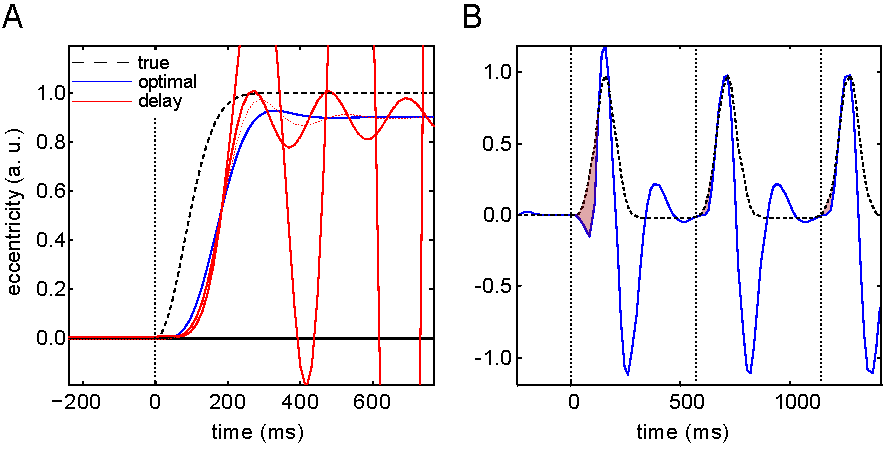
\includegraphics[width=\linewidth]{PerrinetAdamsFriston14.pdf}
}
\caption{\textbf{(A)} Cette figure montre la réponse du traitement
prédictif lors de la simulation du début de la poursuite tout en
compensant les délais sensoriels moteurs, en utilisant un mouvement sigmoïdal simple
d'une cible visuelle. Ici, nous voyons des excursions horizontales de
l'angle oculomoteur (trait bleu foncé). On peut voir clairement le
déplacement initial de la cible qui est supprimé par l'action après
environ $200~\ms$, modélisant un mouvement oculaire prototype de poursuite.
De plus, nous illustrons les effets de l'hypothèse de la connaissance d'un délai
sensori-moteur erroné sur le déclenchement de la poursuite. Avec
un délai sensoriel pur (pointillés rouges), on peut voir
clairement le délai des prédictions sensorielles par rapport aux
entrées réelles. En cas de délai moteur pur (tirets rouges) et de délai sensori-moteur combiné (trait rouge), il y a un
défaut de contrôle optimal avec des fluctuations oscillatoires dans les
trajectoires oculomotrices, qui comme ici peuvent devenir instables. \textbf{(B)}
Cette figure montre la simulation d'une poursuite oculaire lorsque le
mouvement de la cible est hémisinusoïdal, comme dans le cas d'un pendule
qui serait arrêté à chaque demi-cycle à gauche de la verticale (lignes
noires discontinues). Le modèle génératif utilisé ici a été équipé d'un
deuxième niveau hiérarchique qui contient des états cachés, modélisant
le comportement périodique latent des causes (cachées) du mouvement de
la cible. Avec cet ajout, l'amélioration de la précision de poursuite
est apparente dès le début du deuxième cycle de mouvement (aire
rouge ombragée), de façon semblable aux expériences psychophysiques~\citep{Barnes91}. (Reproduit de~\citep{PerrinetAdamsFriston14} selon
les termes de la
\href{https://link.springer.com/article/10.1007/s00422-014-0620-8\#copyrightInformation}{Creative
Commons Attribution License}, © The Authors 2014.)
}
\label{fig:PerrinetAdamsFriston14}
\end{figure}
%-------------------------------------------------------------%
Une perspective intéressante pour étudier le rôle de la dynamique
neurale dans la cognition est d'étendre ce modèle à une description plus
réaliste des contraintes écologiques auxquelles fait face le système
visuel. En effet, le système nerveux central est confronté à des délais
axonaux, tant au niveau sensoriel que moteur. Comme nous l'avons vu dans
l'introduction, il faut environ $50~\ms$ pour que l'image rétinienne
atteigne les aires visuelles impliquées dans la détection de mouvement,
et $50~\ms$ supplémentaires pour atteindre les muscles oculomoteurs et
réaliser l'action~\citep{Kirchner06}. L'un des défis de la
modélisation du système visuo-oculomoteur humain est de comprendre les
mouvements oculaires comme un problème de contrôle moteur optimal avec
des délais axonaux. Prenons l'exemple d'un joueur de tennis qui tente
d'intercepter une balle qui passe à une vitesse (conservatrice) de 20
m/s. La position détectée sur l'espace rétinien correspond à l'instant
où l'image s'est formée sur les photorécepteurs de la rétine, et jusqu'à
ce qu'elle atteigne notre hypothétique aire de perception du mouvement.
À cet instant, la position physique détectée est en fait en décalage d'un
mètre, c'est-à-dire approximativement à une excentricité de 45 degrés.
Cependant, la position au moment de l'émission de la commande du moteur
sera également de 45 degrés \emph{en avant de} sa position physique
actuelle dans l'espace visuel. Par conséquent, si le regard du joueur
n'est pas dirigé vers l'image de la balle sur la rétine mais vers la
balle dans sa position (physique) actuelle, c'est peut-être parce qu'il
prend en compte, de manière anticipée, la distance parcourue par la
balle pendant le délai sensoriel. Alternativement, un contrôle optimal
peut diriger l'action (mouvement futur de l'œil) vers la position
attendue lorsque les commandes motrices atteignent la périphérie
(muscles). Un tel exemple montre que même avec un délai relativement
court, le système visuel est confronté à des perturbations importantes
qui entraînent des choix ambigus. Cette ambiguïté est évidemment un défi
intéressant pour la modélisation du traitement prédictif dans le système
visuel.

En étendant notre précédent cadre de modélisation de la poursuite ocularire~\citep{Adams12},
nous avons observé dans~\citep{PerrinetAdamsFriston14}
que la représentation des états cachés en coordonnées généralisées offre
un moyen simple de compenser les délais sensoriels et moteurs. Une nouveauté de cette
approche est d'inclure les délais dans la dynamique en tirant profit
des coordonnées généralisées. Techniquement, cela définit un opérateur
linéaire sur ces variables qui permet de virtuellement ``voyager dans le temps''
 avec des intervalles
de temps arbitraires, permettant en particulier de représenter les
variables d'état dans le passé (délai sensoriel) ou dans le futur
(délai moteur). Notons que (1) cette représentation est seulement définie à
l'instant présent, (2) qu'elle permet la représentation concomitante de
la précision des variables d'état, et (3) qu'elle permet d'évaluer
l'hypothèse contrefactuelle des états sensoriels (basée sur les états
sensoriels passés) et d'une action qui doit être inférée maintenant,
tout en sachant que celle-ci sera effective après le délai moteur.
L'application d'un tel opérateur au FEP génère une formulation
mathématique légèrement différente et plus complexe. Cependant, il est
important de noter que pour compenser les délais, il n'y a pas de
changement dans la structure du réseau mais seulement dans la façon dont
les poids synaptiques sont réglés (comme nous l'avons fait dans la
première partie de ce programme) :``Neurobiologiquement, l'application
d'opérateurs de délai signifie simplement changer les forces de
connexion synaptique pour prendre différents mélanges de sensations
généralisées et leurs erreurs de prédiction.''~\citep[section 3.1, ma traduction]{PerrinetAdamsFriston14}. En particulier, lorsque l'agent a une
certaine croyance au sujet de ces délais, il peut intégrer de façon
optimale (au sens de Bayes) les croyances internes. Un tel comportement est
toujours régulé par le même type d'équation interne.

Nous avons illustré l'efficacité de ce schéma à l'aide de simulations
neurales des réponses d'initiation à la poursuite, avec et sans
compensation. La figure~\ref{fig:PerrinetAdamsFriston14}-A présente les estimations des probabilités conditionnelles
des états cachés et des causes pendant la simulation de l'initiation de
la poursuite, en utilisant un simple mouvement rectiligne d'une cible visuelle, tout
en compensant les délais sensoriels et moteurs. Ici, nous voyons les
excursions horizontales de l'angle oculomoteur (trait bleu) par rapport à la
position angulaire de la cible (pointillés noirs). %, réelle mais cachée
On peut clairement voir
le déplacement initial de la cible qui est supprimé après
quelques centaines de millisecondes. Cette figure illustre également les
effets des délais sensorimoteurs sur le déclenchement de la poursuite
(lignes rouges) par rapport à l'inférence active compensée (optimale).
Sous les délais sensoriels purs (ligne pointillée), on peut voir
clairement le délai des prédictions sensorielles, par rapport aux
entrées réelles. A noter ici l'échec du contrôle optimal avec des
fluctuations oscillatoires dans les trajectoires oculomotrices, qui
deviennent instables sous l'effet de délais sensorimoteurs combinés.

Il est intéressant de noter que ce modèle s'étend à des trajectoires
visuelles plus complexes. En particulier, il a été démontré que le
regard sera dirigé vers la position physique actuelle de la cible (donc
de manière anticipée) si cette cible suit une trajectoire lisse
(comme un pendule). Plus frappant, c'est également vrai si la
trajectoire est \emph{prévisible}, par exemple pour un pendule derrière
une occlusion statique~\citep{Barnes91,Adams12}. La figure~\ref{fig:PerrinetAdamsFriston14}-B montre la simulation d'une poursuite
en douceur lorsque le mouvement de la cible est hémisinusoïdal, comme
dans le cas d'un pendule qui serait arrêté à chaque demi-cycle, à gauche
de la verticale. Notons que contrairement à l'agent modélisé dans~\citep{Adams12}, cet agent inclut la contrainte biologique
que le traitement sensoriel et moteur sont retardés. Le modèle génératif a
été équipé d'un deuxième niveau hiérarchique qui contient des états
cachés et qui tiennent compte du comportement périodique latent du
mouvement de la cible. On peut clairement voir le déplacement initial de
la cible qui est supprimé après quelques centaines de millisecondes
(aire rouge). L'amélioration de la précision de la poursuite
est apparente au début du deuxième cycle de mouvement, semblable aux
expériences psychophysiques~\citep{Barnes91}. En effet, le
modèle a une représentation interne des causes latentes du mouvement de
la cible qui peut être utilisée même lorsque ces causes ne sont pas
exprimées explicitement (occultées) dans la trajectoire cible. Un
avantage particulier de ce modèle est qu'il fournit une solution pour
l'intégration de l'information passée et future tout en étant gouverné
par des équations différentielles en ligne. Ceci met donc en œuvre une
certaine forme de mémoire temporelle optimale de Bayes.

\subsection{Résumé}
En résumé, nous avons montré ici qu'un cycle complet de perception
/ action pourrait être compris comme un processus prédictif
dans le cadre de l'inférence active~(IA). En particulier, nous avons
montré que de tels modèles pouvaient reproduire la dynamique observée
dans les mouvements oculaires, notamment en introduisant des contraintes
réalistes telles que les délais sensorimoteurs. D'autres modèles
devraient permettre l'introduction de contraintes structurelles encore
plus complexes, comme les lois physiques régissant le mouvement des
objets visuels comme le biais \emph{a priori}~\citep{Damasse18}, la
gravité ou les repères externes~\citep{Kowler14}. Cela peut aider à
synthétiser la plupart des lois qui régissent l'organisation de la
perception visuelle, comme l'a formalisé la théorie de la Gestalt.

\section{Traitement prédictif sur les cartes visuelles}
\label{sec:maps}
Dans un premier temps, nous ayons montré le rôle du traitement prédictif à l'échelle
macroscopique en concevant chaque assemblage neural comme un nœud dans
un graphe de dépendance. Mais existe-t-il des preuves de l'existence de tels
processus à l'échelle de l'espace visuel ?

\subsection{L'effet du flash retardé comme preuve pour le traitement
prédictif dans les cartes
topographiques}
%-------------------------------------------------------------%
\begin{figure}%[b!]
\centering{
\includegraphics[width=\linewidth]{KhoeiMassonPerrinet17.pdf}
}
\caption{
Dans~\citep{KhoeiMassonPerrinet17}, nous proposons un
modèle de traitement prédictif sur une carte topographique. \textbf{(A)}
le modèle consiste en une carte à deux couches : une cible source
d'entrée intègre les informations des capteurs visuels. Par souci de
simplicité, nous n'affichons ici que la dimension horizontale et cette
carte représente sur chaque axe respectivement la position et la
vitesse. En utilisant cette carte comme représentation de la croyance
(ici en utilisant une fonction de distribution de probabilités), il est
possible de projeter cette information sur une deuxième couche cible qui
intègre l'information tout en compensant pour ce délai. Dans
ce cas particulier, la vitesse est positive et donc l'information de
position est transportée vers la droite. \textbf{(B)} Réponse d'un
modèle compensant un délai de $100~\ms$ pour le mouvement d'un point en mouvement.
Représentation de la probabilité inférée de position et de vitesse avec
compensation de délai en fonction des itérations du modèle (temps). Les
couleurs plus foncées dénotent des probabilités plus élevées, tandis
qu'une couleur claire correspond à une estimation improbable. En
particulier, nous nous concentrons sur trois époques particulières le
long de la trajectoire, correspondant à l'initiation, au milieu et à l'extinction.
Le moment de ces trois époques est indiqué par des traits
verticaux en pointillés: en noir pour le temps physique (réel) et en
vert pour l'entrée retardée sachant un délai de $100~\ms$. Voir le texte
pour une interprétation des résultats. (Reproduit de~\citep{KhoeiMassonPerrinet17} selon les termes de la
\href{https://journals.plos.org/ploscompbiol/article?id=10.1371/journal.pcbi.1005068}{Creative
Commons Attribution License}, © The Authors 2017.)
}
\label{fig:KhoeiMassonPerrinet17}
\end{figure}
%-------------------------------------------------------------%

L'\href{https://en.wikipedia.org/wiki/Flash_lag_illusion}{effet
du flash retardé} (Flash-Lag Effect, FLE) est une illusion visuelle populaire pour sa généralité
et sa simplicité. Dans sa forme originale~\citep{MacKay58}, on demande à
l'observateur de fixer une croix centrale sur l'écran
pendant qu'un point traverse l'écran avec un mouvement constant et
horizontal. Lorsqu'il atteint le centre de l'écran, un autre point
clignote brièvement juste en dessous du point en mouvement. Alors qu'ils
sont parfaitement alignés verticalement, le point clignotant est perçu
comme \emph{en retard} par rapport au point en mouvement~\citep{Perrinet19temps}. Cette illusion visuelle a
vu un regain d'intérêt scientifique avec le modèle d'extrapolation de
mouvement~\citep{Nijhawan02,Nijhawan09}. Cependant, d'autres
modèles tels que le modèle de latence différentielle ou la post-diction ont
également été proposés, de sorte que l'on ne savait pas encore clairement
quel est le substrat neural du FLE. Ici, en étendant le modèle de
compensation des délais~\citep{PerrinetAdamsFriston14}, nous
avons défini un modèle de traitement prédictif généralisé sur la
topographie visuelle en utilisant une représentation interne du
mouvement visuel~\citep{Perrinet12pred} qui utilise une diffusion
anisotrope des informations~\ref{fig:KhoeiMassonPerrinet17}-A.

Le modèle que nous avons utilisé pour le FLE peut être utilisé avec
n'importe quelle image. En particulier, un point lumineux isolé évoque une
activité isotrope en expansion puis en contraction, tandis qu'un point
en mouvement peut produire une onde de type soliton qui peut traverser
une occlusion~\citep{Khoei13jpp}. Plus généralement, ce
modèle peut être décrit comme  utilisant le terme d'advection de l'équation de Navier
Stokes qui gouverne la dynamique des fluides. Ainsi,
les solutions à ces équations sont typiquement des ``vagues'' qui se
déplacent sur la carte rétinotopique. Une caractéristique particulière
de ces équations prédictives est qu'elles comprennent un terme d'amplification pour les
mouvements rectilignes. Par conséquent, une fois qu'un objet commence à
être suivi, sa position est prévue dans le futur, de sorte que la
position et la vitesse sont mieux estimées. Au contraire, un point qui
se déplace sur une trajectoire imprévisible est éliminée par le système.
Ceci explique certains des comportements non linéaires, de type
binaire, qui sont expliqués par ce modèle~\citep{Perrinet12pred}. Il est
particulièrement intéressant à ce stade de comprendre si un tel modèle
s'étend à d'autres stimuli ou si l'on peut préciser son implémentation
neurale.

Appliquée à l'image du FLE, l'activité dans le modèle montre trois
phases différentes, voir~\ref{fig:KhoeiMassonPerrinet17}-B. Premièrement, il y a une
augmentation rapide de la précision de la cible après la première
apparition du point mobile (à $300~\ms$). En cohérence avec
l'\href{https://en.wikipedia.org/wiki/Fröhlich_effect}{effet Fröhlich}~\citep{Jancke10}, le début de la trajectoire est vu ``en avant'' par rapport à sa
position physique. Pendant la deuxième phase, le point en mouvement est
suivi efficacement car sa vitesse et sa position sont correctement
déduites. Comme observé dans l'illusion, l'extrapolation de mouvement prédit correctement la
position actuelle et la position suit la position physique réelle du
point (ligne pointillée noire) : Le point est perçu en avant de la trajectoire retardée du point (ligne
pointillée verte).
De façon équivalente, le flash est perçu en retard par rapport au point en mouvement.
Enfin, la troisième phase correspond à
la fin du mouvement. Le point en mouvement disparaît et
l'activité correspondante disparaît dans la couche source à $t=900~\ms$.
Cependant, entre $t=800~\ms$ et $t=900~\ms$, la position du point a été
extrapolée et prédite avant la position finale. À $t=900~\ms$, alors que
l'information de mouvement est absente, l'information de position est
encore transitoirement cohérente et extrapolée à l'aide d'une large
distribution de vitesses centrée au préalable : Bien qu'elle soit moins
précise, cette position du point à la fin du flash n'est donc pas perçue comme étant en avant du flash, mais \emph{rétrospectivement} dû à cette nouvelle information.

\subsection{Corrélat neural du mouvement apparent}
Appliquons une approche similaire à une autre illusion visuelle :
Lorsque deux points stationnaires clignotent à des positions et à des
moments rapprochés l'un de l'autre, l'observateur peut percevoir une
sensation de mouvement. Ce processus transforme la présentation d'un motif
discret en un motif continu et est à la base des processus qui nous font percevoir au cinéma une image animée alors que nos yeux ne ressentent qu'une succession rapide d'images statiques.
Cette illusion visuelle est appelée
\href{https://en.wikipedia.org/wiki/Beta_movement}{mouvement apparent}
et peut persister sur une distance spatiale relativement longue (supérieure à la
taille caractéristique de la RF d'un neurone dans le cortex visuel
primaire, V1). Comme dans l'étude ci-dessus pour le FLE, nous pensons que ce
mouvement apparent à longue portée (long-range Apparent Motion, lrAM) peut s'expliquer par des
processus prédictifs. En raison des caractéristiques dynamiques du lrAM,
une implémentation neurale de cette illusion peut consister en la
propagation d'informations visuelles par des interactions
intra-corticales. En particulier, ces interactions latérales peuvent
évoquer des vagues d'activité dans V1 qui peuvent moduler l'intégration de
l'information sensorielle provenant des connexions thalamo-corticales.
Une perspective intéressante est donc d'enregistrer l'activité neurale
lors de la présentation du stimulus lrAM. Ceci permet d'évaluer
quantitativement pourquoi la superposition de deux points comme dans le
lrAM est ``plus'' que la somme des deux points isolés.

Dans une étude récente~\citep{Chemla19}, nous avons utilisé la VSDI
pour enregistrer l'activité du cortex visuel primaire (V1) de macaques
éveillés. Y a-t-il une différence entre la réponse au point unique et
celle aux deux points ? En effet, les enregistrements VSD permettent
d'enregistrer l'activité de populations de neurones V1 qui sont
approximativement à l'échelle d'une colonne corticale. De plus, la
réponse enregistrée est assez rapide pour saisir la dynamique du
stimulus lrAM. Les enregistrements montrent que lorsque l'activité
évoquée par le second point atteint V1, une onde corticale suppressive se
propage vers la vague rétinotopique évoquée par le premier point. Cela a
été mis en évidence en comparant statistiquement la réponse du cerveau à
la réponse des deux points isolés. En particulier, nous avons constaté
que grâce à cette onde suppressive, l'activité du stimulus cérébral
était plus précise, ce qui suggère que cette onde suppressive pourrait
servir d'étape de traitement prédictive pour être lue dans les aires
corticales en amont.

En particulier, nous avons constaté que l'activité que nous avons
enregistrée était bien décrite par un modèle de champ moyen utilisant un
contrôle de gain dynamique. Qualitativement, ce modèle reproduit la
propagation de l'activité sur le cortex. Il est important de noter que
ce modèle a permis de montrer que l'activité observée était mieux
ajustée lorsque la vitesse des connexions latérales dans le champ moyen
était d'environ $1 m/s$, une vitesse de propagation qui est de l'ordre de
celle mesurée pour les connexions intra-corticales dans le cortex visuel
primaire (pour une revue, voir~\citep{Muller18}). Un modèle plus
fonctionnel (probabiliste) a également montré que la vague
corticale suppressive permettait de lever l'ambiguïté sur le stimulus en supprimant
les alternatives improbables. Par conséquent,
(1) les interactions latérales sont essentielles pour générer des vagues d'activité
en mouvement à la surface du cortex et (2) ces vagues aident à affiner la représentation
du stimulus en entrée. Cela correspond à la mise en œuvre d'un processus
prédictif utilisant une connaissance \emph{a priori} des objets visuels
en mouvement régulier.

\subsection{Résumé}
En résumé, nous avons vu qu'il est possible d'étendre le traitement
prédictif aux cartes topographiques. En particulier, les calculs qui en
résultent sont particulièrement adaptés à la vision. Nous avons montré
(voir~\ref{fig:KhoeiMassonPerrinet17}) un modèle qui représente (à un instant donné) différentes
variables (ici ``Source'' et ``Cible''). Dans un modèle plus réaliste,
l'activité neurale est plus susceptible de former des représentations
intermédiaires entre les représentations passées, présentes et futures~\citep{Glaser18} et à différents niveaux d'adaptation comme
l'illustre le stimulus lrAM~\citep{Chemla19}. En conséquence, de
tels processus sont observés phénoménologiquement comme la propagation
de l'information neurale tangentiellement à la surface corticale,
modulant dynamiquement les flux convergeant sur l'aire corticale (``feed-forward'' vs ``feed-back''). En
particulier, la question reste ouverte de savoir si de tels calculs
neuraux pourraient être mis en œuvre par des vagues d'activité sur la
surface corticale~\citep{Muller18}.

\section{Problèmes ouverts des processus visuels prédictifs}
\label{sec:spikes}
Dans la section~\ref{sec:ai}, nous avons étudié la dynamique du traitement prédictif à
l'échelle macroscopique, c'est-à-dire en considérant les aires
(corticales) comme des noeuds d'un graphe de dépendance. En section~\ref{sec:maps},
nous avons étendu ces modèles à la topographie de chaque aire visuelle. À une échelle
encore plus fine que cette échelle mésoscopique intermédiaire se trouve
l'échelle microscopique des cellules neurales. Pour mieux
comprendre les mécanismes du traitement prédictif, je propose d'affiner
maintenant la granularité de la modélisation à l'échelle neurale
pour définir une hiérarchie de cartes de micro-circuits prototypiques. En
particulier, en plus de la nature asynchrone de la représentation
neurale que nous avons explorée ci-dessus, la communication entre
neurones a la propriété d'être basée sur des événements. En effet, la
grande majorité des cellules neurales à travers le monde vivant
communiquent en utilisant des impulsions courtes et prototypiques
appelées potentiels d'action ou \emph{spikes}. Dans cette section, nous
proposons trois problèmes ouverts qui sont soulevés lors de la
modélisation de tels réseaux de neurones impulsionnels (Spiking Neural Networks, SNN), en particulier dans le contexte du traitement prédictif.

\subsection{Les défis de la représentation de l'information visuelle
dans les réseaux de neurones impulsionnel
(SNN)}
Après les premières générations d'ANN, les algorithmes actuels
d'apprentissage machine tels que les algorithmes d'apprentissage profond
(Deep Learning, DL) constituent une percée qui a formé une deuxième génération d'ANNs.
Les SNN constituent une troisième génération potentielle~\citep{Ghosh09}. En effet, la représentation événementielle présente de
nombreux avantages par rapport aux ANNs classiques. Par exemple, au lieu de
répéter tous les calculs ­pour chaque couche, canal et pixel d'un ANN
hiérarchique, et pour lesquels des GPU gourmands en énergie sont
nécessaires, il suffit dans un SNN d'effectuer les calculs seulement sur les événements
émis par des unités actives (au moment du spike). En particulier, un domaine de
recherche en plein essor consiste à développer des matériels dédiés,
comme les puces neuromorphiques, qui permettraient d'étendre le volume
effectif des calculs au-delà des dernières générations de
semi-conducteurs classiques (CPU, GPU) qui atteignent les limites de la
loi de Moore.

La nature discrète de l'adressage des neurones, d'une part, et la nature
analogique de la synchronisation des spikes, d'autre part, sont
essentielles dans ce nouveau type de représentation. Des résultats
notables utilisant de telles architectures ont été obtenus dans la
classification en temps réel et la fusion de capteurs~\citep{Oconnor13} et dans la reconnaissance de formes~\citep{Lagorce17}. En
effet, une propriété importante des SNNs est la capacité d'encoder
dynamiquement une variable interne latente (le potentiel de membrane en
neuro-physiologie) et d'émettre un spike quand (et seulement quand) un
seuil défini en interne est atteint. Ceci définit chaque neurone spikant
comme un intégrateur (similaire aux neurones classiques), mais aussi
potentiellement comme un détecteur de synchronisation~\citep{Perrinet02}.
Cette capacité à moduler le traitement en fonction de la synchronisation
relative des spikes présynaptiques constitue un nouveau paradigme pour les
calculs neuraux~\citep{Paugam12}. Cela montre en
particulier que l'équilibre du flux des spikes excitateurs et inhibiteurs
entrants est crucial pour maximiser l'efficacité de ces SNN~\citep{Hansel12}.

\subsection{Le rôle des vagues d'activité corticales dans le traitement
dynamique de l'information
visuelle}
Un autre point crucial dans le décryptage des mécanismes de traitement
prédictif est donné par l'anatomie fonctionnelle. En effet, dans le
cortex visuel primaire (V1) comme dans les autres aires corticales, le
réseau neural est très majoritairement récurrent avec un nombre médian de $10000$
connexions par neurone. Étonnamment, $95 \%$ de ces connexions se
produisent dans un rayon de $2 mm$ (singe macaque)~\citep{Markov13}.
Cela suggère qu'une majorité de ressources neurales est consacrée aux
communications intra-régionales. Un rôle fonctionnel supposé de ce
réseau dense est de générer des vagues d'activité qui modulent la force
et la dynamique de l'activité neurale ``feed-forward''~\citep{Muller18}. Nous avons vu son rôle potentiel dans la désambiguïsation du
mouvement~\citep{Chemla19} et il a également été démontré qu'il
facilite l'accumulation progressive de l'information visuelle~\citep{Bringuier99}. Auparavant, nous avons modélisé avec succès un tel
processus prédictif~\citep{Perrinet12pred,Khoei13jpp,KhoeiMassonPerrinet17}, et l'avons mis en œuvre dans un SNN~\citep{Kaplan13}.

Un ``Saint Graal'' dans cette direction est de trouver des micro-circuits
canoniques pour le codage prédictif~\citep{Bastos12}. Cela découle
de l'observation qu'à travers les espèces et les aires, le cortex semble
suivre une structure prototypique en couches. Dans le cas particulier de
V1, alors que l'entrée thalamique atteint principalement la couche
granulaire (intermédiaire), un flux de feed-forward se propage
principalement aux couches efférentes à travers les couches
supra-granulaires tandis que le feed-back est en majorité conduit  par les
couches infra-granulaires. Cette ségrégation anatomique pourrait
correspondre à différents types de signaux dans le codage prédictif,
respectivement des états attendus et des erreurs de prédiction~\citep{Bastos12}. De tels micro-circuits de base ont été utilisés pour
expliquer la réponse des neurones V1 aux scènes naturelles~\citep{Kremkow16} en utilisant un mécanisme push-pull. Des réseaux fonctionnels utilisant un apprentissage dépendant du temps des spikes ont aussi été utilisés pour expliquer des réponses obtenues chez le chat~\citep{Ladret19sfn}. Il n'en demeure pas moins
qu'il est difficile de savoir comment un tel circuit peut émerger de principes computationnels généraux.

\subsection{Propriétés intégratives des aires corticales}
%-------------------------------------------------------------%
\begin{figure}%[b!]
\centering{
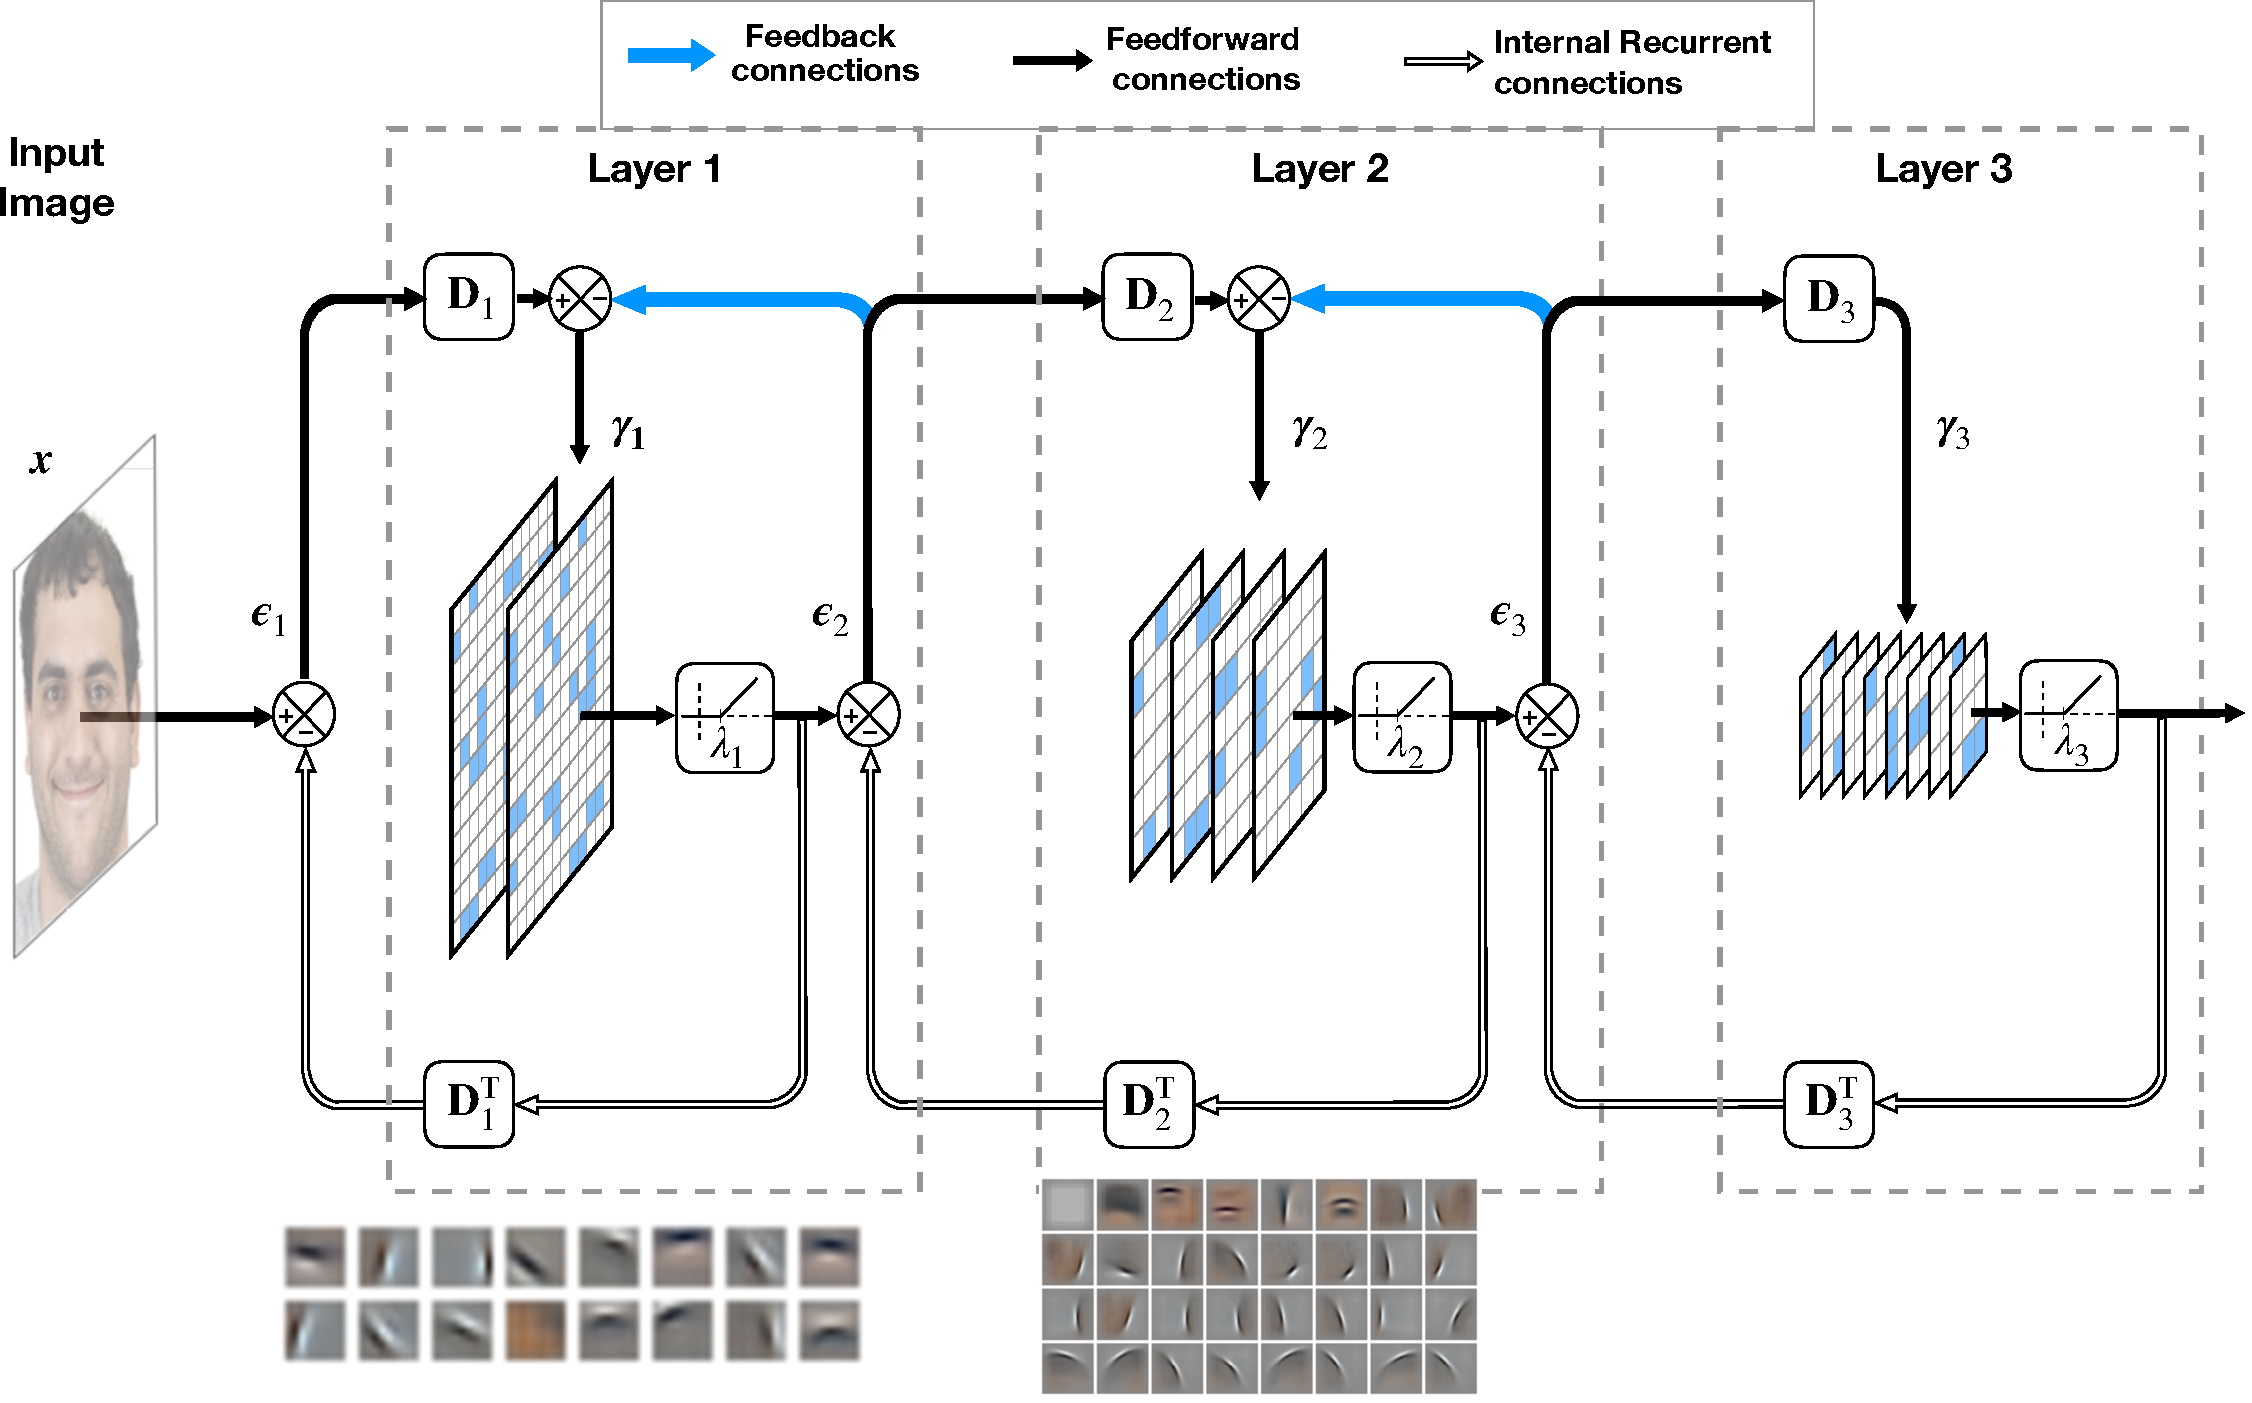
\includegraphics[width=\linewidth]{BoutinFranciosiniChavaneRuffierPerrinet19.pdf}
}
\caption{
Dans~\citep{BoutinFranciosiniChavaneRuffierPerrinet19}, nous proposons un
modèle de traitement hiérarchique de l'information visuelle (ici de 3 couches).
De façon similaire à des réseaux de neurones convolutionnels classiques,
chaque couche est constituée de canaux auxquels sont attribués des champs récepteurs.
Toutefois, contrairement aux réseaux classiques, l'apprentissage est ici bio-mimétique,
c'est-à-dire qu'au lieu d'opérer une retro-propagation (globale) du gradient,
les opérations sont toutes locales et s'opèrent de proche en proche.
Cet apprentissage non-supervisé est possible par l'introduction
d'une contrainte de régularisation assurant la parcimonie de la représentation.
On observe l'émergence de champs récepteurs sensibles à des bords orientés dans la première couche,
de façon similaire à ce qui est observé dans le cortex visuel primaire.
De façon plus surprenante, quand on apprend le réseau sur une base d'images de visages,
on observe l'émergence de cellules sensible à des composantes indépendantes : bouche, yeux, contours allongés,~\ldots
%(Reproduit de~\citep{BoutinFranciosiniChavaneRuffierPerrinet19} selon les termes de la \href{https://journals.plos.org/ploscompbiol/article?id=10.1371/journal.pcbi.1005068}{Creative Commons Attribution License}, © The Authors 2017.)
}
\label{fig:BoutinFranciosiniChavaneRuffierPerrinet19}
\end{figure}
%-------------------------------------------------------------%
Une autre perspective intéressante est la nature intégrative des calculs
neuraux. Bien que l'on croit souvent que les neurones représentent la
combinaison de caractéristiques visuelles, ce n'est en général pas
correct~\citep{Tring18}. Au lieu de cela, il a été constaté que
l'activité peut devenir plus précise à mesure que les caractéristiques
visuelles s'accumulent. Par exemple,~\citep{Baudot13} a montré que
les neurones de l'aire 17 du chat réagissent plus sélectivement
lorsqu'ils présentent des images naturelles (qui consistent localement
en une somme de bords) qu'à un seul bord isolé. Récemment,
nous avons montré qu'un résultat similaire peut se produire chez les rongeurs dès
la rétine~\citep{Ravello19}. Sur le plan comportemental, cela correspond
également à l'observation chez l'homme que des textures plus complexes
entraînent des mouvements oculaires plus robustes~\citep{Simoncini12}. Ces phénomènes sont conformes au principe du traitement prédictif
selon lequel, en accumulant des informations cohérentes, la probabilité
\emph{a posteriori} (et donc la réponse du système) devient plus
précise.

Fait frappant, cela se traduit dans l'activité neurale par le fait que,
pour un ensemble plus cohérent d'entrées sensorielles, l'activité neurale de la
population est plus ``parcimonieux'' (en anglais, ``sparse'')~\citep{Vinje02,Baudot13}.
Cela s'expliquait déjà par le modèle de codage prédictif de~\citep{Rao99} et mis en œuvre dans~\citep{Kremkow16} par exemple. Il
est important de noter que le principe de codage parcimonieux est lui-même
suffisant pour (1) expliquer de façon raisonnée une grande partie des
mécanismes de contrôle du gain~\citep{Heeger17}  et (2) guider
l'apprentissage de la connectivité dans une population de neurones,
comme dans V1~\citep{Olshausen97,Perrinet10shl,Perrinet15bicv,Perrinet19hulk}. Cela aide
à résoudre un problème important, à savoir que le système est
auto-organisé et que l'apprentissage de la connectivité ne doit pas être
supervisé. Ainsi, les règles de plasticité qui devraient être élaborées
dans les SNN devraient utiliser des principes directeurs similaires.

Cependant, il nous manque encore des modèles réalistes d'un tel
traitement prédictif visuel. Nous avons construit un modèle simplifié
capable de traiter des images statiques~\citep{BoutinFranciosiniChavaneRuffierPerrinet19}. Il s'agit
d'un réseau neural convolutionnel multicouche, où chaque couche comprend à la fois un
mécanisme intra-cortical récursif pour générer des représentations
parcimonieuses et la possibilité pour chaque couche d'intégrer des informations
(feedback) provenant d'une couche de niveau supérieur, voir Figure~\ref{fig:BoutinFranciosiniChavaneRuffierPerrinet19}.
La principale
nouveauté de ce réseau est qu'il permet l'apprentissage non supervisé
des noyaux convolutionnels à chaque couche. Comparés aux réseaux de neurones
convolutionnels classiques tels que ceux que l'on trouve couramment dans les
architectures d'apprentissage profond, nous avons constaté que les
noyaux émergents étaient plus interprétables : Par exemple, en apprenant
sur une classe d'images de visages humains, nous avons observé dans la
deuxième couche différents neurones sensibles aux caractéristiques du
visage comme les yeux, la bouche ou le nez.
C'est similaire à ce que
l'on trouve dans l'aire corticale du \href{https://fr.wikipedia.org/wiki/Lobule_fusiforme}{lobule fusiforme}, mais d'autres simulations
sont nécessaires pour valider l'émergence de cette représentation.
Nous avons aussi observé que les connections en retour, en ``feedback''
avaient une importance significative sur cette émergence~\citep{BoutinFranciosiniRuffierPerrinet20feedback}.
Toutefois, ces simulations sont intensives en calcul et interdisent leur
extension à des flux dynamiques sur des architectures informatiques conventionnelles. Une
traduction de cet algorithme en un réseau neural impulsionnel serait donc
très bénéfique et permettrait de l'appliquer à un flux dynamique
d'images.

\section{Résumé et conclusions}
En résumé, nous avons examiné dans ce programme de recherche différents modèles de
codage prédictif appliqués à la vision. Nous avons vu à l'échelle
macroscopique le rôle de la dynamique à l'aide de l'inférence active
(voir section~\ref{sec:ai}). En étendant ce modèle à une carte rétinotopique, nous
pourrions décrire une onde progressive fonctionnelle pour améliorer la sélectivité à des
stimuli visuels (voir section~\ref{sec:maps}). Cependant, nous avons également montré
une limite de ces modèles à l'échelle microscopique (voir section~\ref{sec:spikes}). En
particulier, on ne comprend pas encore, au niveau de la cellule unique,
comment (1) l'information est représentée dans l'activité impulsionnelle, (2)
quel est le rôle fonctionnel des vagues d'activité sur les surfaces
corticales, (3) si un principe d'efficacité commun (comme un codage
parcimonieux) pouvait être utilisé pour guider l'organisation de ces réseaux
hautement récurrents dans un circuit universel unique.

Pour approfondir nos connaissances du traitement prédictif en vision
(voir section~\ref{sec:spikes}), il semble donc nécessaire de pouvoir mettre en œuvre
des SNN à grande échelle mettant en œuvre des processus visuels
complexes. Cependant, les trois différentes échelles anatomiques que
nous avons mises en évidence ci-dessus (feed-forward, latéral, feedback)
semblent être étroitement couplées et peuvent être difficiles à
modéliser séparément. Plus généralement, c'est également vrai pour les
échelles que nous avons définies, depuis le macroscopique, jusqu'au mésoscopique
et au microscopique. Il est donc très difficile de produire des modèles
assez simples pour nous aider à comprendre le traitement sous-jacent~\citep{Varoquaux19,Brette19}. Par exemple, après les avoir
déduits des principes d'optimisation, tous les modèles que nous avons
présentés ici sont préconnectés : Les hyper-paramètres contrôlant
l'interconnexion des neurones sont fixes. Bien que nous ayons fourni des
simulations montrant le rôle de ces hyperparamètres, il semble
nécessaire de mieux comprendre leurs effets relatifs. %En particulier,
%nous pensons que de telles architectures auto-organisées pourraient
%définir le temps comme un processus prédictif de synchronisation de
%variables émergentes aux multiples niveaux du traitement visuel.

En effet, une théorie normative du traitement prédictif ne devrait pas
seulement fournir une solution possible (un modèle donné avec un
ensemble d'hyperparamètres) mais aussi explorer \emph{toutes les
solutions possibles}. Une première méthodologie consiste à avoir une
compréhension complète de l'ensemble des modèles à l'aide de l'analyse
mathématique. Cependant, cela devient impossible pour des systèmes aussi
complexes et l'utilisation d'hypothèses simplificatrices conduit souvent
à une complexité superficielle. Un autre moyen consiste à élaborer des
stratégies d'adaptation pour explorer l'espace fonctionnel de différents
modèles. Ceci peut par exemple être développé à l'aide de techniques
d'apprentissage machine telles que la descente stochastique de gradient
couramment utilisée dans l'apprentissage profond. Une autre solution
prometteuse consiste à explorer des stratégies d'adaptation inspirées de
la biologie. Celles-ci existent à différentes échelles
temporelles, allant des mécanismes d'adaptation rapide, à un
apprentissage plus lent des connexions, ou à l'évolution à long terme
des hyper-paramètres. En particulier, on ne comprend pas encore tout à
fait comment implanter dans les SNNs une plasticité dépendante du temps de
spike. Cela pose un défi futur dans notre compréhension de la science des
processus prédictifs en vision qui définira mon prochain programme de recherche.
%
\printbibliography
\end{document} %
